\setlength{\footskip}{8mm}

\chapter{Methodology}
\label{ch:methodology}

\section{System Design}
Figure 3.1 shows the design of the final product. 
\begin{figure}[!ht]
  \centering
  \includegraphics[scale=0.5]{figures/design.png}  
  \caption[Design of the final product.]{Design of the final product.}
  \label{fig:Design}
\end{figure}
\FloatBarrier

\section{Solution overview}

The goal of this research is to build and evaluate a system able to detect our three researchers in the surveillance videos of a mall, as shown in the previous section. My solution is composed of five steps.
\begin{itemize}
\item Initially, we have a database of videos.\newline
\item Then, these videos are processed to extract the faces of every person appearing in them. We have now a database of faces.\newline
\item From this database, I extract training patterns for the learning and test processes.\newline
\item A model is trained to recognize our researchers or an existing model is acquired from available models.\newline
\item The model is tested on our database of videos.
\end{itemize}

\section{Solution Design}

Figure 3.2 presents two main ideas. In blue, the steps described in the above section are shown. In green, the solutions used to go from one step to the next are described.\newline
\begin{figure}[!ht]
  \centering
  \includegraphics[scale=0.7]{figures/methodology.png}  
  \caption[An overview of the global design of the study.]{An overview of the global design of the study.}
  \label{fig:Methodology}
\end{figure}
\FloatBarrier

\section{Database}
As said in the introduction, deep learning algorithms were applied to perform face recognition in a video surveillance system. A database of surveillance videos was required to generate a training set and a test set for our model.
The database that was used for the learning process is a set of 14 videos recorded in the MBK Shopping Center in Bangkok. The duration of the videos is variable, from a minute to around 3 minutes and 30 seconds. Three of the researchers of our laboratory appear in the videos, walking in the mall like any other person.

\section{Raw Database of Faces}

A C++ algorithm using OpenCV (Bradski, 2000) provided in Algorithm 1 was used for face detection.

\begin{algorithm}[H]
 \For{each video in the database}{
 \For{each frame N of the current video}{
 	  Detect all the faces of the frame N\;
  	Save the P-th detection in \enquote{Database/video/FrameNFaceP.jpg}\;
  }
  }
 \caption{Face detection algorithm}
\end{algorithm}

The algorithm used for face detection uses a machine learning process called Haar feature-based cascade classifiers, described by Viola and Jones (2001).

Once the process is over, a \enquote{Database} directory is created with one directory for each video. In each directory, all of the faces are saved as JPEG files.

\begin{figure}[!ht]
  \centering
  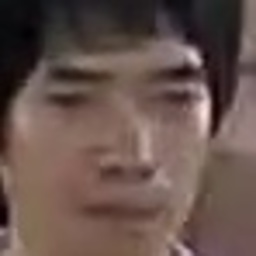
\includegraphics[scale=0.7]{figures/face1.jpg}
  
\includegraphics[scale=0.7]{figures/face2.jpg}
  \caption[An example of two faces extracted from the surveillance system. On the left, one of the target individuals. On the right, a typical customer of the shopping center.]{An example of two faces extracted from the surveillance system.}
  \label{fig:face}
\end{figure}

\section{Creation of database files}

The framework that will be presented in the next section requires two files to work: a \texttt{train.txt} file and a \texttt{test.txt} file. Their role is trivially linked to their name in a supervised learning process.

\subsection{Case of direct face identification}
 In the case of direct face identification, each of the \texttt{train.txt} and \texttt{test.txt} files share the same structure:

\begin{verbatim}
/adress/of/the/training/image1.jpg label1\newline
/adress/of/the/training/image2.jpg label2\newline
...\newline
/adress/of/the/training/imageN.jpg labelN
\end{verbatim}

The labels are assigned automatically using the simple tracking method described in the next subsection.

The labels of the researchers were obtained by automatically tracking then manually merging tracks of the same researcher in different video segments.

\subsection{Face tracking}

\begin{algorithm}[H]
\For{each video in the database}{
 \For{each frame of the current video}{
  Detect all the faces of the frame N\;
 \For{each face of the current frame}{
    \If{there is a face detected in the three previous frames whose distance with the current face is inferior to the size of the face}{
    The label L of the current face := The label of the nearest of the faces of the three previous frames\;
    Save the detected face in \enquote{Database/video/LabelLFrameNFaceP.jpg}\;
    }
    \Else{}{
    The label L of the current face := Biggest label given until now + 1
    Save the detected face in \enquote{Database/video/LabelLFrameNFaceP.jpg}\;
    }
  }
  }
  }
 \caption{Automatic Labeling Algorithm}
\end{algorithm}

A representation of the final database is given below:


\begin{figure}[!ht]
  \centering
  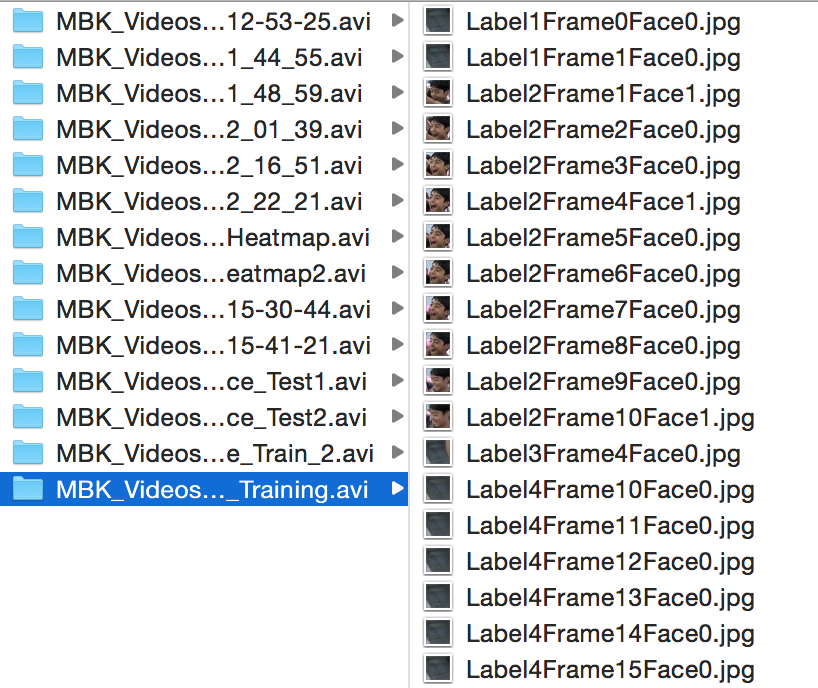
\includegraphics[scale=0.7]{figures/databaserepresentation.png}  
  \caption[The database after automatic labeling.]{The database after automatic labeling.}
  \protect\label{fig:Siamese}
\end{figure}
\FloatBarrier
\end{itemize}

\subsection{Case of a \enquote{Same/Not same} model}

In the case of a \enquote{Same/Not same} model, the problem was a bit different. A slightly unusual structure is best for this model. The solution is to generate two files for training and two files for testing. Let's name them \texttt{train1.txt}, \texttt{train2.txt}, and \texttt{test1.txt} and \texttt{test2.txt}. Their individual structure are as explained before.

\blockquote{/adress/of/the/training/image1.jpg label1\newline
/adress/of/the/training/image2.jpg label2\newline
...\newline
/adress/of/the/training/imageN.jpg labelN}

In line K, train1.txt and train2.txt contain respectively \enquote{address/to/file1K.jpg labelK} and \enquote{address/to/file2K.jpg labelK}. The labels are identical. However, the images are different. If both the images represent the same person, the label will be 1, and 0 otherwise. \texttt{test1.txt} and \texttt{test2.txt} will work the same way. Only one of the two labels are used for the supervised learning, the other one, being identical, is not used. The syntax of the training and testing files being fixed with Caffe, this solution seems to be the most adapted to the problem encountered with the \enquote{Same/Not Same} models. The fact that two face images are considered as different or identical is determined by the face tracking algorithm described above.


\subsection{Conclusion}
It was a feasible task to create a series of Python scripts that run one after the other to create the required \textt{train.txt} and \texttt{test.txt} files. These python scripts are indirectly launched through bash scripts. A README file will be provided to explain which commands to type and which options to select to generate the required files from the database.\\

The purpose of the designed architecture is to make those scripts reusable for any new database and generalizable for an arbitrary number of labels. If a user provides another database of videos, and follows the process described in the \texttt{README} file, the required \texttt{train.txt} and \texttt{test.txt} files will be generated, and the models presented in the next section can be used for learning or testing directly on these data.

\section{Model}

\subsection{Framework}
The chosen deep learning framework for this study is Caffe (Jia et al., 2014).\\

\subsection{Strategy}
Different strategies have been considered for this modelisation. As explained in the previous chapter, there are two usual schemes for face recognition.
\begin{itemize}
\item The first one is the \enquote{same/not same} or \enquote{face verification} scheme. The idea is to readjust the Siamese network described by Lecun et al. (2005) to our particular dataset.\newline
\item The second scheme is direct face identification. For this purpose, the idea is to modify the last layer of a state-of-the-art deep neural network architecture for face identification. The output of this last modified layer should be binary. Either the input image represents one of our researchers --- in practice, a criminal ----, or it does not. The previous layers should already be trained, and the training should be done in the last layer only.
\end{itemize}
\subsection{The learning process with Caffe}

The Caffe framework requires several files to train a model.
\begin{itemize}
\item First, \texttt{train.txt} and \texttt{test.txt} files, which give paths to all images with corresponding labels.\newline
\item Second, a \texttt{train\_test.prototxt} file that describes the architecture of the network. This file is written with protobuf. According to the \texttt{README} file available on the project's GitHub site, \blockquote{Protocol Buffers (a.k.a., protobuf) are Google's language-neutral, platform-neutral, extensible mechanism for serializing structured data.}. Figure \ref{fig:logreg} shows how a logistic regression classifier is easily defined in a train\_test.prototxt file with Caffe.

\begin{figure}[!ht]
  \centering
  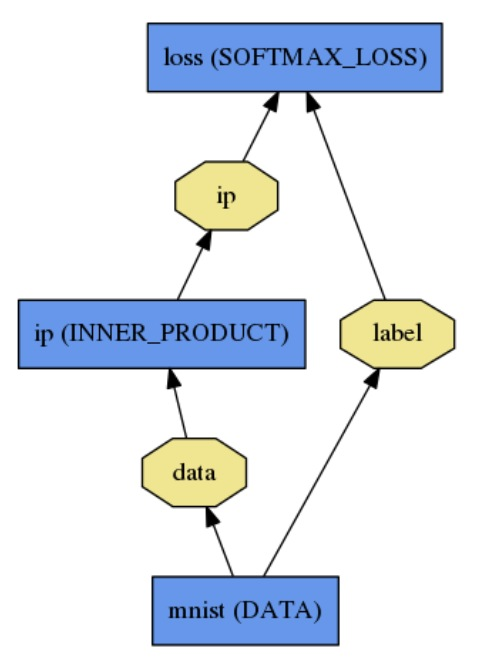
\includegraphics[scale=0.7]{figures/logreg.jpg}
  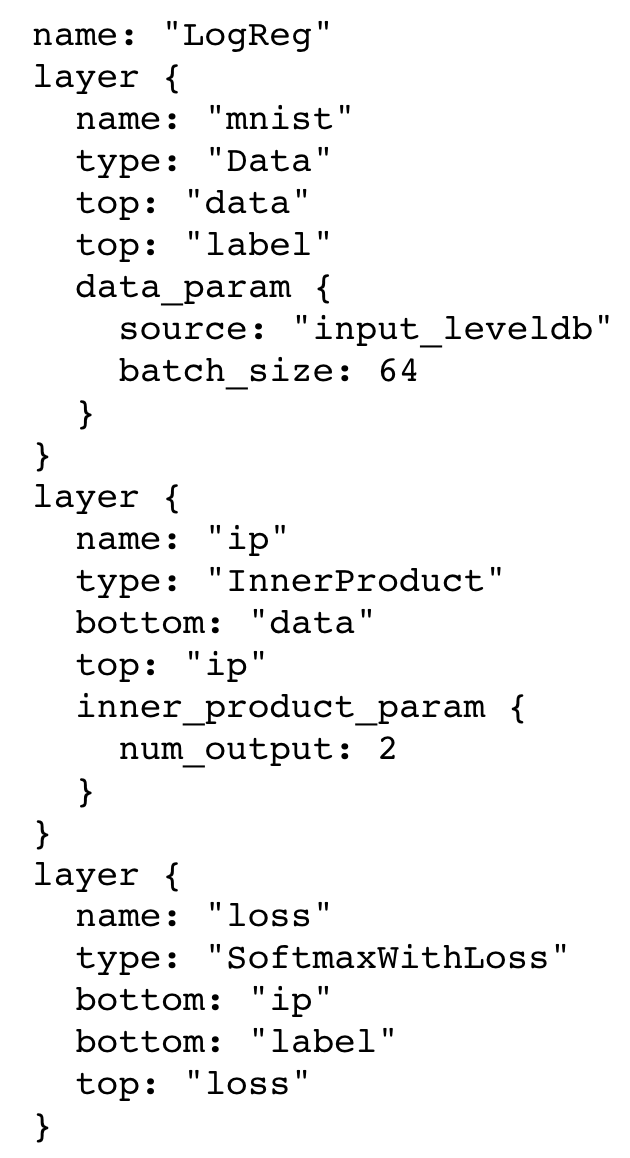
\includegraphics[scale=0.4]{figures/logregfile.png}
  \caption[Logistic regression classifier definition with Caffe. Extracted from the official website of the framework.]{Logistic regression classifier definition with Caffe. Extracted from the official website of the framework.}
  \label{fig:logreg}
\end{figure}

\FloatBarrier

\item Third, a \texttt{solver.prototxt} file, which contains information on the batch size or on the variables related to the used loss function.
\end{itemize}

The learning process produces two files: A \texttt{.caffemodel} and a \texttt{.solverstate}. These files are used to store the value of the parameters of the designed model after a number of steps of learning chosen in the \texttt{.solverstate} file.

\section{Testing}

As we just said, the output of a face identification model should be binary. A Python script to test the accuracy of the model can be written with no difficulty. On the contrary, the input of a Siamese network is two images and the output can be interpreted as an energy. This energy is high for two images representing two different people and low otherwise (in some models, it is the opposite). A threshold on this energy has to be determined to make classification possible with the network. Thus, before any test, a script had to be written to determine a good threshold on the training set. This script was written using pycaffe, the caffe model for python. Then, and only then could the tests be done.